\chapter{Planificación}
\minitoc
\label{chap:planificacion}
\vspace{0.5cm}

%%%%%%%%%%%%%%%%%%%%%%%%%%%%%%%%%%%%%%%%%%%%%%%%%%%%%%%%%%%%%%%%%%%%%%%%%%%%%%%%
% Objetivo: Exponer la planificación del PFC.                                  %
%%%%%%%%%%%%%%%%%%%%%%%%%%%%%%%%%%%%%%%%%%%%%%%%%%%%%%%%%%%%%%%%%%%%%%%%%%%%%%%%

\lettrine{N}{este} capítulo exporase a planificación do proxecto: como se levou a
cabo, que ciclo de vida se escolleu e por que, como quedou a planificación
inicial, etc.

O motivo de poñer a planificación nun capítulo a parte previo ó resto dos
capítulos do proxecto, é dar unha visión global dos mesmos coa finalidade de
que se entenda o porqué desa distribución.

\section{Ciclo de vida}

O ciclo de vida escollido foi o \textbf{ciclo de vida en espiral}
\cite{TemarioES} (figura \ref{figura:CicloVidaEspiral}) por ser o que mellor se
adapta ás características deste proxecto.

\begin{figure}[htbp]
 \centering
 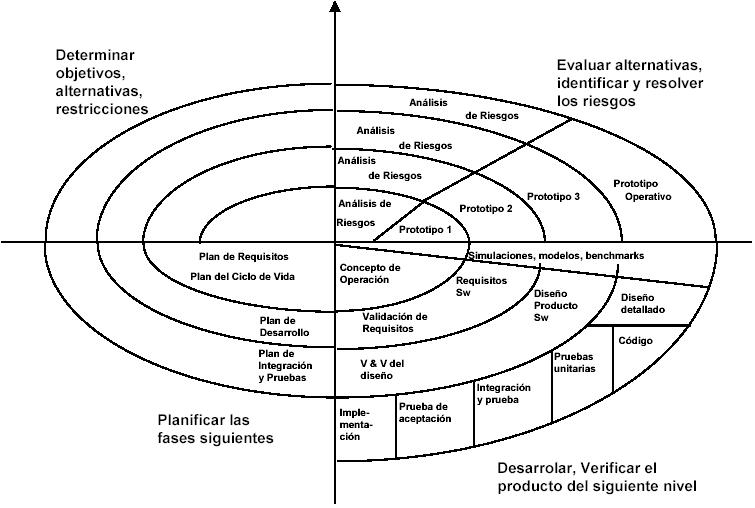
\includegraphics[scale=0.6,keepaspectratio=true]{./imagenes/espiral.jpg}
 % espiral.jpg: 755x508 pixel, 96dpi, 19.98x13.44 cm, bb=0 0 566 381
 \caption[Ciclo de vida en espiral]{Ciclo de vida en espiral \cite{TemarioES}.}
 \label{figura:CicloVidaEspiral}
\end{figure}

Dito ciclo de vida conta coas seguintes características:

\begin{itemize}
 \item Permite combinar a natureza interactiva de construcción de prototipos
       cos aspectos controlados e sistemáticos do modelo en cascada.
 \item Pon especial énfase na análise dos riscos.
 \item O software desenvólvese nunha serie de versións incrementais:
       \begin{itemize}
        \item Durante as primeiras iteracións, a versión incremental será un
              modelo en papel ou un prototipo.
        \item Durante as últimas iteracións, prodúcense versións cada vez máis
              completas do sistema.
        \item A idea básica é que cada fase (volta na espiral) establece os
              seguintes pasos:
              \begin{itemize}
               \item Determinación de obxectivos, alternativas e restriccións.
               \item Avaliación de alternativas (considerando análise de
                     riscos).
               \item Desenvolvemento do seguinte nivel de producto.
               \item Planificación da seguinte fase (ciclo en espiral).
              \end{itemize}
        \item Cada ciclo (volta) na espiral representa unha fase do proceso de
              desenvolvemento.
              \begin{itemize}
               \item Por ilo, o ciclo máis interno correspóndese coa
                     viabilidade do sistema.
               \item O seguinte, coa análise de requisitos e así sucesivamente.
              \end{itemize}
        \item Non hai fases fixas no modelo. O modelo adáptase ás necesidades
              que xordan en cada proxecto.
        \item Os bloques de deseño, codificación e probas execútanse de forma
              secuencial para a entrega dunha características iniciais
              operativas.
        \item Despois dilo, vólvese revisar o producto e cómo mellorar/ampliar
              as súas características operativas. O producto actualízase,
              obtendo un prototipo operativo “posto ó día” que serve de
              demostración e validación.
        \item O sistema pasa por un proceso actualizado de desenvolvemento en
              cascada que finalmente obtén unha nova versión do producto.
        \item Esquema básico (espiral de 4 pasos):
              \begin{enumerate}
               \item 1º ciclo:
                     \begin{itemize}
                      \item Determinación de:
                            \begin{itemize}
                             \item Obxectivos.
                             \item Alternativas.
                             \item Restriccións.
                            \end{itemize}
                      \item Avaliación de alternativas e resolución de riscos:
                            \begin{itemize}
                             \item Análise de riscos.
                             \item Prototipo 1.
                            \end{itemize}
                      \item Desenvolvemento e validación do seguinte nivel de
                            producto:
                            \begin{itemize}
                             \item Concepto de operación.
                            \end{itemize}
                      \item Planificación da próxima fase (ciclo):
                            \begin{itemize}
                             \item Planificación de requisitos.
                             \item Planificación do ciclo de vida.
                            \end{itemize}
                     \end{itemize}
               \item 2º ciclo:
                     \begin{itemize}
                      \item Determinación de:
                            \begin{itemize}
                             \item Obxectivos.
                             \item Alternativas.
                             \item Restriccións.
                            \end{itemize}
                      \item Avaliación de alternativas e resolución de riscos:
                            \begin{itemize}
                             \item Análise de riscos.
                             \item Prototipo 2.
                            \end{itemize}
                      \item Desenvolvemento e validación do seguinte nivel de producto:
                            \begin{itemize}
                             \item Simulacións, modelos e programas de proba.
                             \item Requisitos do software.
                             \item Validación de requisitos.
                            \end{itemize}
                      \item Planificación da próxima fase (ciclo):
                            \begin{itemize}
                             \item Planificación do deseño.
                            \end{itemize}
                     \end{itemize}
               \item 3º ciclo:
                     \begin{itemize}
                      \item Determinación de:
                            \begin{itemize}
                             \item Obxectivos.
                             \item Alternativas.
                             \item Restriccións.
                            \end{itemize}
                      \item Avaliación de alternativas e resolución de riscos:
                            \begin{itemize}
                             \item Análise de riscos.
                             \item Prototipo 3.
                            \end{itemize}
                      \item Desenvolvemento e validación do seguinte nivel de producto:
                            \begin{itemize}
                             \item Simulacións, modelos e programas de proba.
                             \item Deseño do producto software.
                             \item Verificación e validación do deseño.
                            \end{itemize}
                      \item Planificación da próxima fase (ciclo):
                            \begin{itemize}
                             \item Planificación do desenvolvemento.
                            \end{itemize}
                     \end{itemize}
               \item 4º ciclo:
                     \begin{itemize}
                      \item Determinación de:
                            \begin{itemize}
                             \item Obxectivos.
                             \item Alternativas.
                             \item Restriccións.
                            \end{itemize}
                      \item Avaliación de alternativas e resolución de riscos:
                            \begin{itemize}
                             \item Análise de riscos.
                             \item Prototipado operacional.
                            \end{itemize}
                      \item Desenvolvemento e validación do seguinte nivel de producto:
                            \begin{itemize}
                             \item Simulacións, modelos e programas de proba.
                             \item Deseño detallado.
                             \item Codificación.
                             \item Probas de unidade.
                             \item Integración e probas.
                             \item Probas de aceptación.
                             \item Implantación.
                            \end{itemize}
                     \end{itemize}
              \end{enumerate}
       \end{itemize}
\end{itemize}

As vantaxes que presenta este ciclo de vida son as seguintes:

\begin{itemize}
 \item Permite adaptar o proceso de desenvolvemento ás necesidades cambiantes
       do proxecto e ó coñecemento que se vai adquirindo.
 \item Permite o manexo de prototipos, ligándoos coa análise de riscos.
 \item Xestiona explicitamente os riscos.
\end{itemize}

Pero tamén ten os seus inconvintes:

\begin{itemize}
 \item Require dunha considerable habilidade para a consideración do risco.
 \item O modelo é relativamente novo e non se manexou tanto coma os anteriores.
\end{itemize}

Como se pode deducir claramente da sección de vantaxes, este ciclo de vida
adáptase moi ben ó tipo de proxecto do que estamos a falar.

\section{Descrición das tarefas}

Aplicando o exposto no apartado anterior sobre o ciclo de vida, o seguinte foi
adaptalo ás necesidades do proxecto e definir cada unha das tarefas.

Neste apartado descríbense tódalas tarefas folla listadas na planificación, así
coma o traballo realizado en cada unha das mesmas.

\begin{enumerate}
 \item Análise de viabilidade:
       \begin{itemize}
        \item Determinación de:
              \begin{itemize}
               \item Obxectivos: estableceranse os obxectivos da fase de
                     análise de viabilidade do proxecto.
               \item Alternativas: estableceranse posibles alternativas a eses
                     obxectivos, aplicables no caso de que estes non se poidan
                     cumprir.
               \item Restriccións: estableceranse restriccións aplicables a
                     ditos obxectivos.
              \end{itemize}
        \item Avaliación de alternativas e resolución de riscos:
              \begin{itemize}
               \item Análise de riscos: determinaranse os riscos que comportan
                     as distintas alternativas e as súas posibles solucións.
               \item Prototipo 1: realizarase un primeiro prototipo que nos
                     permita intuir como será o producto final.
              \end{itemize}
        \item Desenvolvemento e validación do seguinte nivel de
              producto:
              \begin{itemize}
               \item Concepto de operación: trata de definir de maneira
                     conceptual cómo se operará co producto, aclarando que é o
                     que se pretende conseguir máis exactamente, de xeito que
                     sexa máis sinxelo obter os requisitos nunha fase
                     posterior.
              \end{itemize}
        \item Planificación da próxima fase (ciclo):
              \begin{itemize}
               \item Planificación de requisitos: estableceranse as tarefas da
                     seguinte fase da planificación do proxecto, a análise de
                     requisitos.
               \item Planificación do ciclo de vida: establecerase o ciclo de
                     vida a empregar, xustificando o seu uso.
              \end{itemize}
       \end{itemize}
 \item Análise de requisitos:
       \begin{itemize}
        \item Determinación de:
              \begin{itemize}
               \item Obxectivos: estableceranse os obxectivos da fase de
                     análise de requisitos do proxecto.
               \item Alternativas: estableceranse posibles alternativas a eses
                     obxectivos, aplicables no caso de que estes non se poidan
                     cumprir.
               \item Restriccións: estableceranse restriccións aplicables a
                     ditos obxectivos.
              \end{itemize}
        \item Avaliación de alternativas e resolución de riscos:
              \begin{itemize}
               \item Análise de riscos: determinaranse os riscos que comportan
                     as distintas alternativas e as súas posibles solucións.
               \item Prototipo 2: realizarase un segundo prototipo que nos
                     permita obter de maneira sinxela os requisitos do
                     producto.
              \end{itemize}
        \item Desenvolvemento e validación do seguinte nivel de producto:
              \begin{itemize}
               \item Simulacións, modelos e programas de proba: estableceranse
                     unha serie de probas a realizar sobre o prototipo anterior
                     unha vez obtidos os requisitos.
               \item Requisitos hardware, software e económicos: 
                     \begin{itemize}
                      \item Extracción de requisitos propia: estableceranse os
                            requisitos do producto por parte do proxectando.
                      \item Extracción de requisitos por parte de expertos:
                            estableceranse os requisitos do producto por parte
                            de expertos preseleccionados.
                      \item Extracción de requisitos a través dos usuarios:
                            Estableceranse os requisitos do producto por parte
                            de usuarios anónimos.
                     \end{itemize}
               \item Validación de requisitos: cruzaranse tódolos datos obtidos
                     durante a obtención de requisitos e validarase por parte
                     do proxectando e dos expertos que o producto é correcto
                     (fai o que se lle pide), empregando as probas definidas
                     anteriormente.
              \end{itemize}
        \item Planificación da próxima fase (ciclo):
              \begin{itemize}
               \item Planificación do deseño: estableceranse as tarefas da
                     seguinte fase da planificación do proxecto, o deseño.
              \end{itemize}
       \end{itemize}
 \item Deseño:
       \begin{itemize}
        \item Determinación de:
              \begin{itemize}
               \item Obxectivos: estableceranse os obxectivos da fase de deseño
                     do proxecto.
               \item Alternativas: estableceranse posibles alternativas a eses
                     obxectivos, aplicables no caso de que estes non se poidan
                     cumprir.
               \item Restriccións: estableceranse restriccións aplicables a
                     ditos obxectivos.
              \end{itemize}
        \item Avaliación de alternativas e resolución de riscos:
              \begin{itemize}
               \item Análise de riscos: determinaranse os riscos que comportan
                     as distintas alternativas e as súas posibles solucións.
               \item Prototipo 3:
                     \begin{itemize}
                      \item Prototipo hardware: realizarase un prototipo
                            hardware mediante ferramentas software.
                      \item Prototipo software: realizarase un terceiro
                            prototipo, baseado no prototipo da fase anterior
                            integrando tódolos cambios precisos para pasar a
                            validación de requisitos.
                     \end{itemize}
              \end{itemize}
        \item Desenvolvemento e validación do seguinte nivel de producto:
              \begin{itemize}
               \item Simulacións, modelos e programas de proba: estableceranse
                     unha serie de probas a realizar sobre o prototipo
                     anterior, co fin de determinar se o deseño posterior é
                     correcto.
               \item Deseño do producto hardware e software.
                     \begin{itemize}
                      \item Deseño do producto hardware: baseándose no
                            prototipo hardware anterior, realizarase un deseño
                            formal do producto hardware.
                      \item Deseño do producto software: baseándose no
                            prototipo software anterior, realizarase un deseño
                            formal do producto software.
                     \end{itemize}
               \item Verificación e validación do deseño: verificarase que o
                     deseño se fixo correctamente (que se axusta ás
                     especificacións) e que é correcto (fai o que se lle pide).
              \end{itemize}
        \item Planificación da próxima fase (ciclo):
              \begin{itemize}
               \item Planificación do desenvolvemento: estableceranse as
                     tarefas da seguinte fase da planificación do proxecto, o
                     desenvolvemento.
              \end{itemize}
       \end{itemize}
 \item Desenvolvemento:
       \begin{itemize}
        \item Determinación de:
              \begin{itemize}
               \item Obxectivos: estableceranse os obxectivos da fase de
                     desenvolvemento do proxecto.
               \item Alternativas: estableceranse posibles alternativas a eses
                     obxectivos, aplicables no caso de que estes non se poidan
                     cumprir.
               \item Restriccións: estableceranse restriccións aplicables a
                     ditos obxectivos.
              \end{itemize}
        \item Avaliación de alternativas e resolución de riscos:
              \begin{itemize}
               \item Análise de riscos: determinaranse os riscos que comportan
                     as distintas alternativas e as súas posibles solucións.
               \item Prototipado operacional.
                     \begin{itemize}
                      \item Prototipo hardware:
                            \begin{itemize}
                             \item Integración do hardware: seguindo o
                                   prototipo hardware realizado por software da
                                   fase anterior e o posterior deseño hardware,
                                   realizarase unha versión física do mesmo.
                             \item Encapsulamento do hardware: unha vez
                                   integrado o hardware será preciso
                                   encapsulalo de forma que sexa sinxelo
                                   interactuar con el.
                            \end{itemize}
                      \item Prototipo software:
                            \begin{itemize}
                             \item Desenvolvemento do prototipo: elaboración
                                   dun prototipo software completo (incluindo a
                                   parte do controlador hardware).
                             \item Gravación dos samples: elaboración, partindo
                                   de cero, dunha fonte de sons de calidade
                                   para empregar co producto.
                            \end{itemize}
                     \end{itemize}
              \end{itemize}
        \item Desenvolvemento e validación do seguinte nivel de producto:
              \begin{itemize}
               \item Simulacións, modelos e programas de proba: estableceranse
                     unha serie de probas a realizar sobre o prototipo
                     anterior, co fin de determinar se o deseño posterior é
                     correcto.
               \item Deseño detallado:
                     \begin{itemize}
                      \item Deseño hardware: ampliación do deseño hardware da
                            fase anterior.
                      \item Deseño software: ampliación do deseño software da
                            fase anterior.
                     \end{itemize}
               \item Ensamblado e codificación:
                     \begin{itemize}
                      \item Ensamblado: integración do hardware e do
                            encapsulamento.
                      \item Codificación: desenvolvemento completo software.
                     \end{itemize}
               \item Probas de unidade: testeo das distintas partes do producto
                     facendo uso das probas definidas previamente.
               \item Integración e probas: fusión de tódalas partes do producto
                     nunha única e posterior testeo facendo uso das probas
                     definidas previamente.
               \item Probas de aceptación: verificación e validación do
                     producto por parte de expertos.
               \item Implantación: simulación da implantación do producto nun
                     sistema limpo e preparado para o mesmo. Por exemplo, unha
                     máquina virtual creada expresamente para a defensa do
                     proxecto.
              \end{itemize}
       \end{itemize}
\end{enumerate}

\section{Xestión do proxecto}

Para poder manexar as tarefas anteriores era necesario facer uso dunha
ferramenta de xestión de proxectos, comunmente coñecida como \textbf{xestor de
proxectos} ou planificador. \\

Tendo en conta a filosofía do proxecto, o correcto era empregar un xestor de
proxectos libre. Facendo un pouco de investigación e preguntando a profesionais
con experiencia no uso dos mesmos, preseleccionáronse varios de entre os moitos
existentes, para o seu posterior estudio:

\begin{itemize}
 \item OpenProj \cite{OpenProj}
 \item Planner \cite{Planner}
 \item GanttProject \cite{GanttProject}
 \item LibrePlan \cite{LibrePlan}
\end{itemize}

Nunha primeira avaliación superficial, \textit{Planner} e \textit{GanttProject}
arroxaron unha imaxe de demasiado básicos, mentres que \textit{LibrePlan}
permite xestionar proxectos complexos, co inconvinte de ter unha interface máis
lenta que as alternativas xa mencionadas. \\

Foi nesta primeira avaliación onde \textit{OpenProj} destacou sobre o resto por
quedarse xusto en medio: lixeiro, completo e moi similar (por non dicir un
clon) ó \textit{MS Project} \cite{MSProject}, planificador xa manexado polo
proxectando e, polo tanto, reducindo a curva de aprendizaxe e o tempo invertido
en dominalo. \\

Escolleuse entón \textit{OpenProj} coma primeira opción, pero logo dunha serie
de incidencias que se comentan no capítulo \ref{chap:conclusiones}, a opción
final empregada foi \textbf{LibrePlan}. \\

Para rematar, facer notar que por motivos de dispoñibilidade de tempo do
proxectando (estudos, traballo, etc.) decidiuse empregar un calendario de media
xornada para o proxecto.

\section{Planificación inicial}

Pouco a pouco fóronse introducindo todos os datos ata dar coa
\textbf{planificación inicial}, cun total de \textbf{688 horas} de traballo
planificadas. \\

A continuación amósase a planificación inicial (figuras
\ref{figura:PlanificacionInicial1} e \ref{figura:PlanificacionInicial2})
recortada coas tarefas organizadas de forma arbórea. Dada a súa extensión,
iranse desglosando por ciclos nos seguintes capítulos para facilitar a súa
comprensión. \\

Pode consultarse a planificación completa (incluíndo as dependencias entre
tarefas) no apéndice \ref{chap:planificacion-completa}.

\begin{figure}[htbp]
 \centering
 %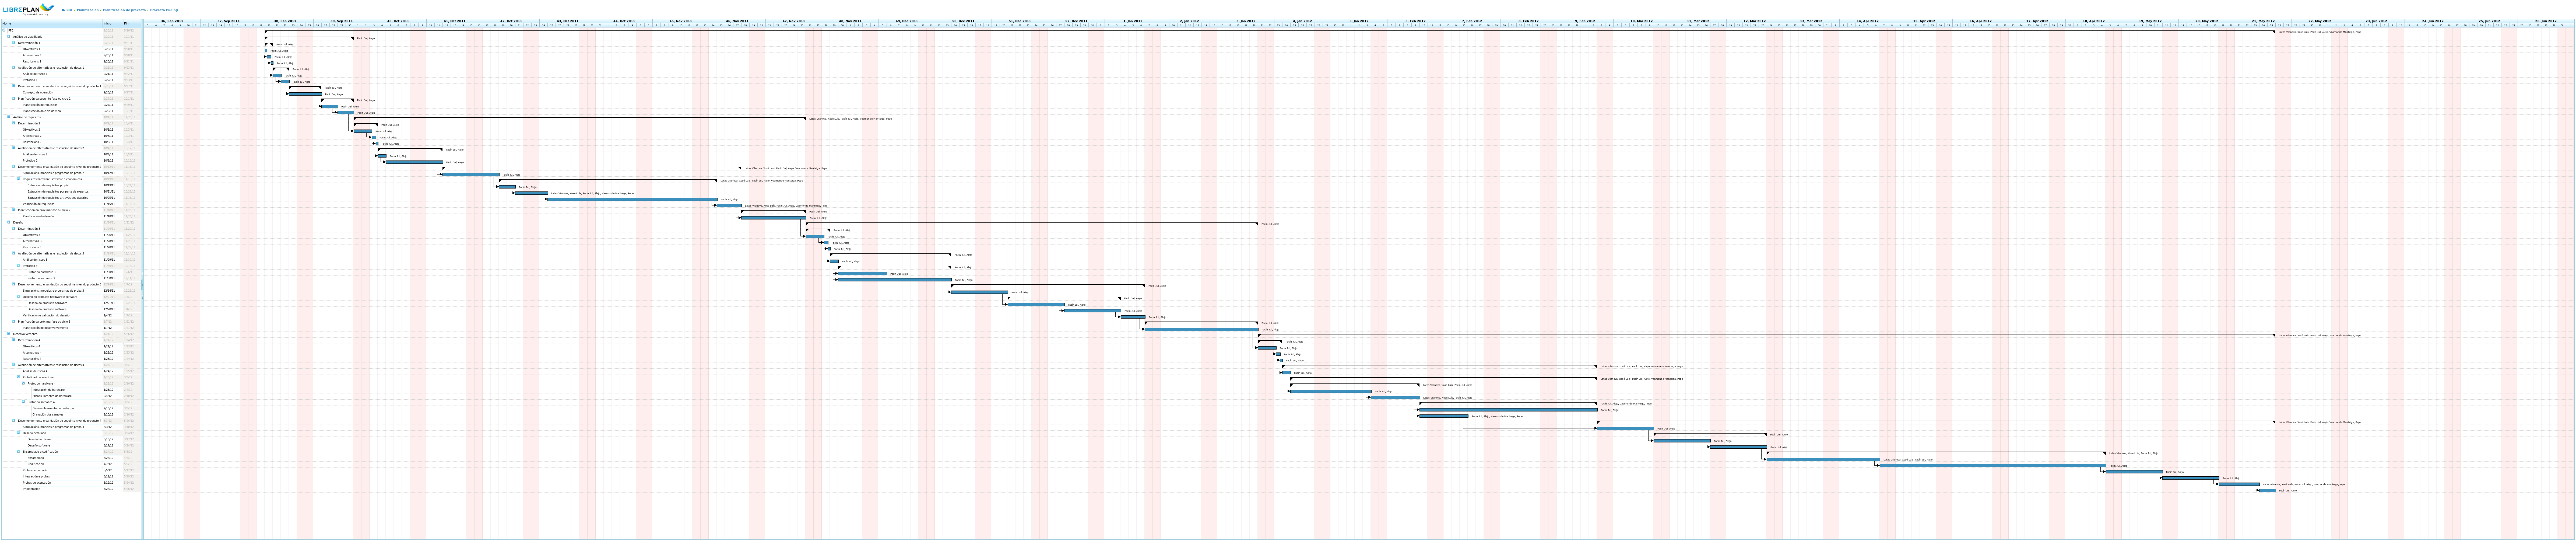
\includegraphics[scale=0.08,angle=90,keepaspectratio=true]{./imagenes/planificacion-inicial.png}
 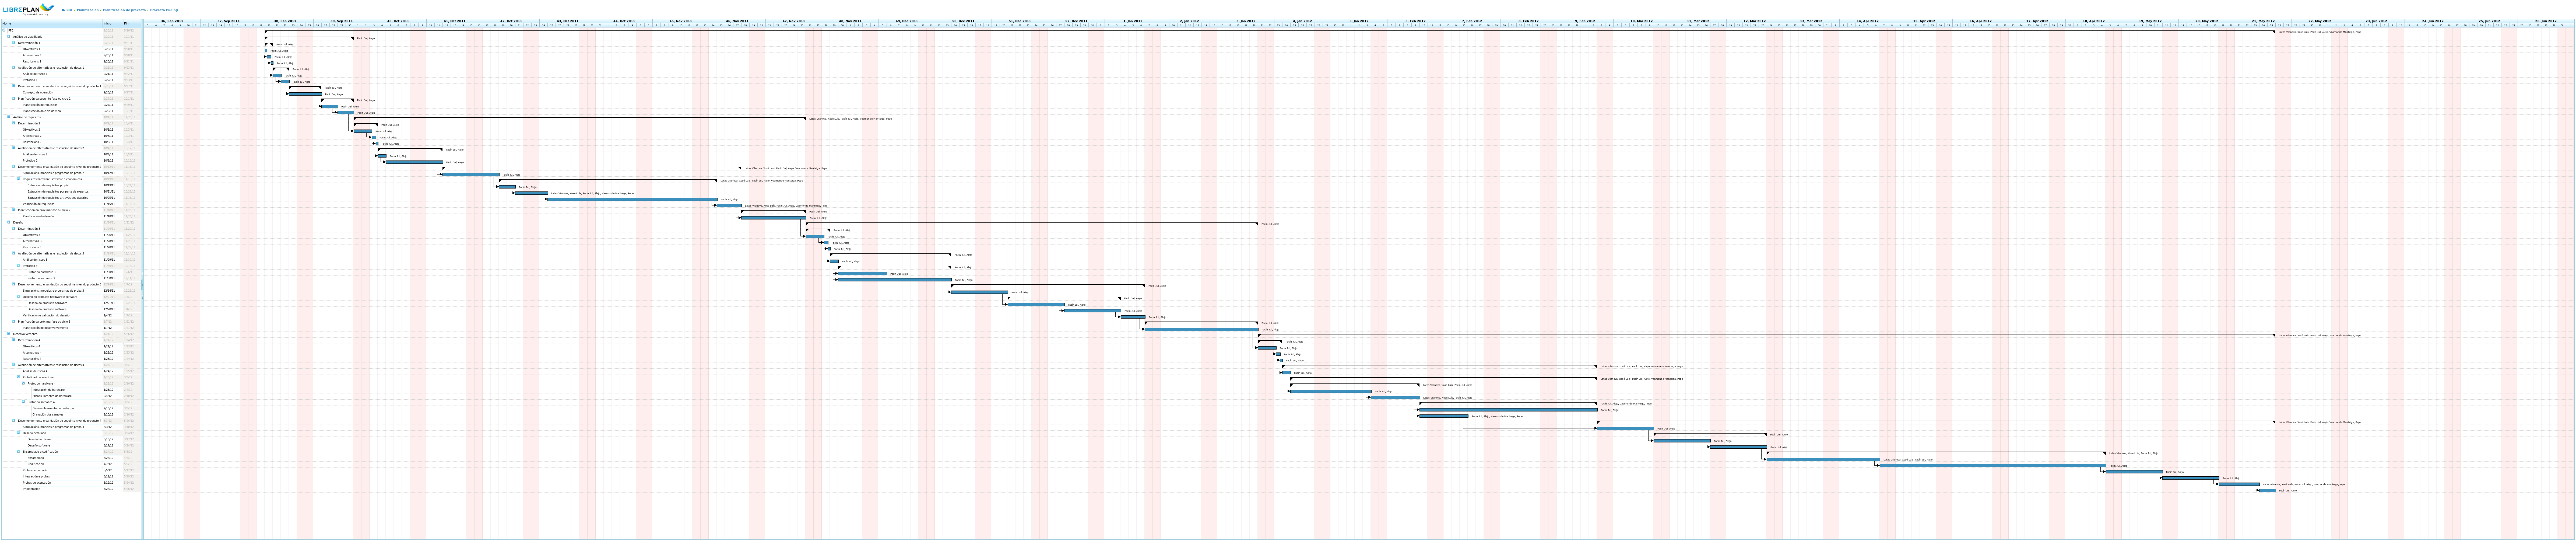
\includegraphics[trim=0 20cm 230cm 0,clip=true,scale=0.6,keepaspectratio=true]{./imagenes/planificacion-inicial.png}
 % planificacion-inicial.png: 9571x2035 pixel, 100dpi, 243.10x51.69 cm, bb=0 0 6891 1465
 \caption[Planificación inicial (1/2)]{Planificación inicial (1/2) \cite{LibrePlan}.}
 \label{figura:PlanificacionInicial1}
\end{figure}

\begin{figure}[htbp]
 \centering
 %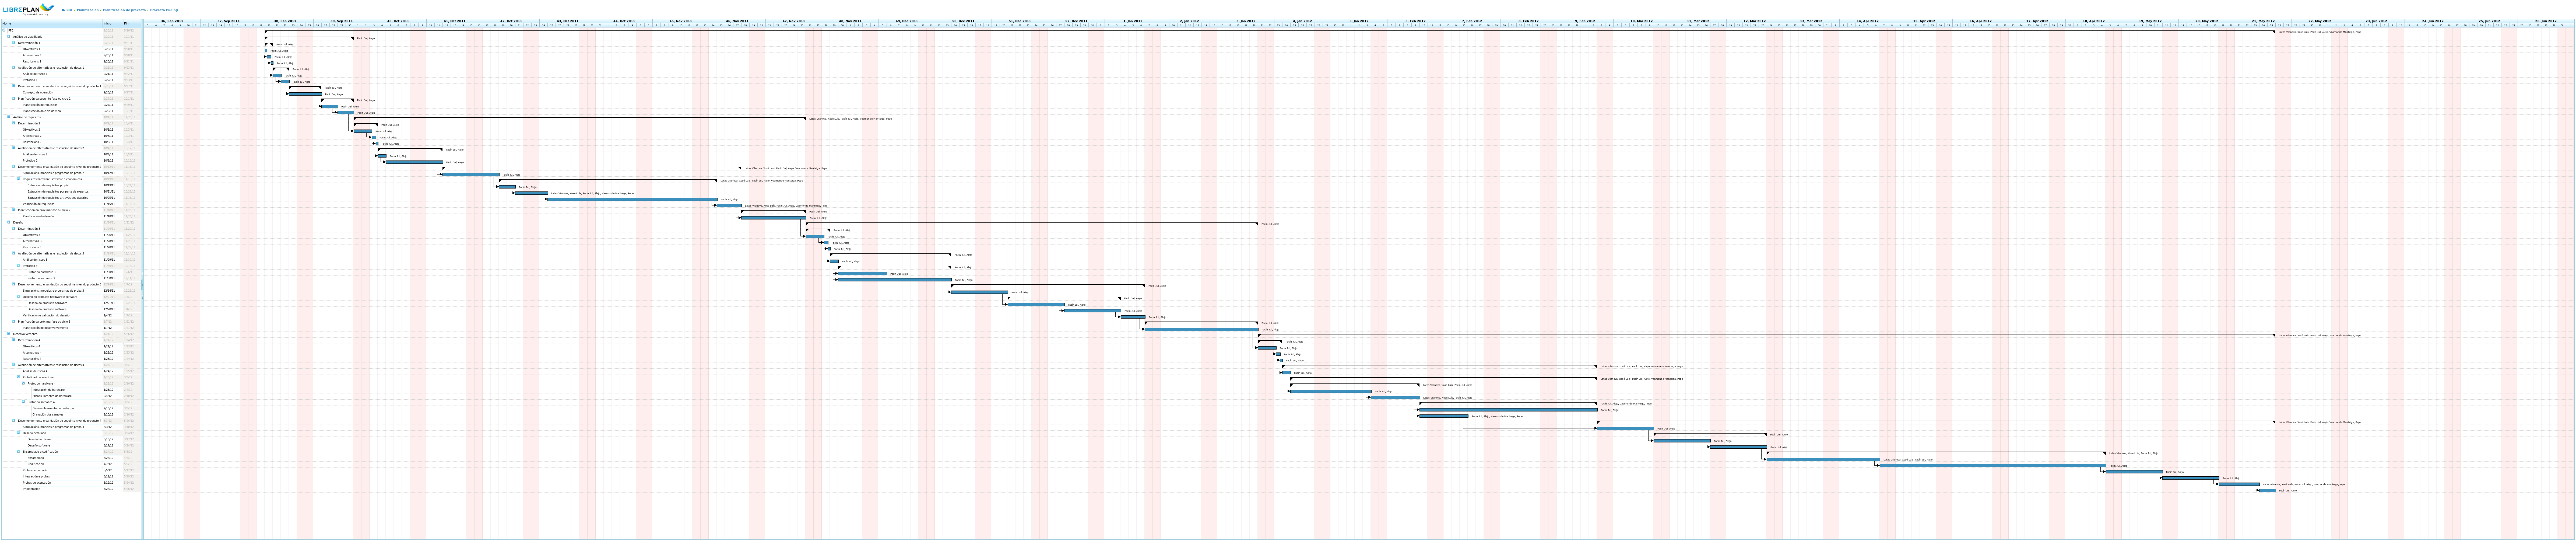
\includegraphics[scale=0.08,angle=90,keepaspectratio=true]{./imagenes/planificacion-inicial.png}
 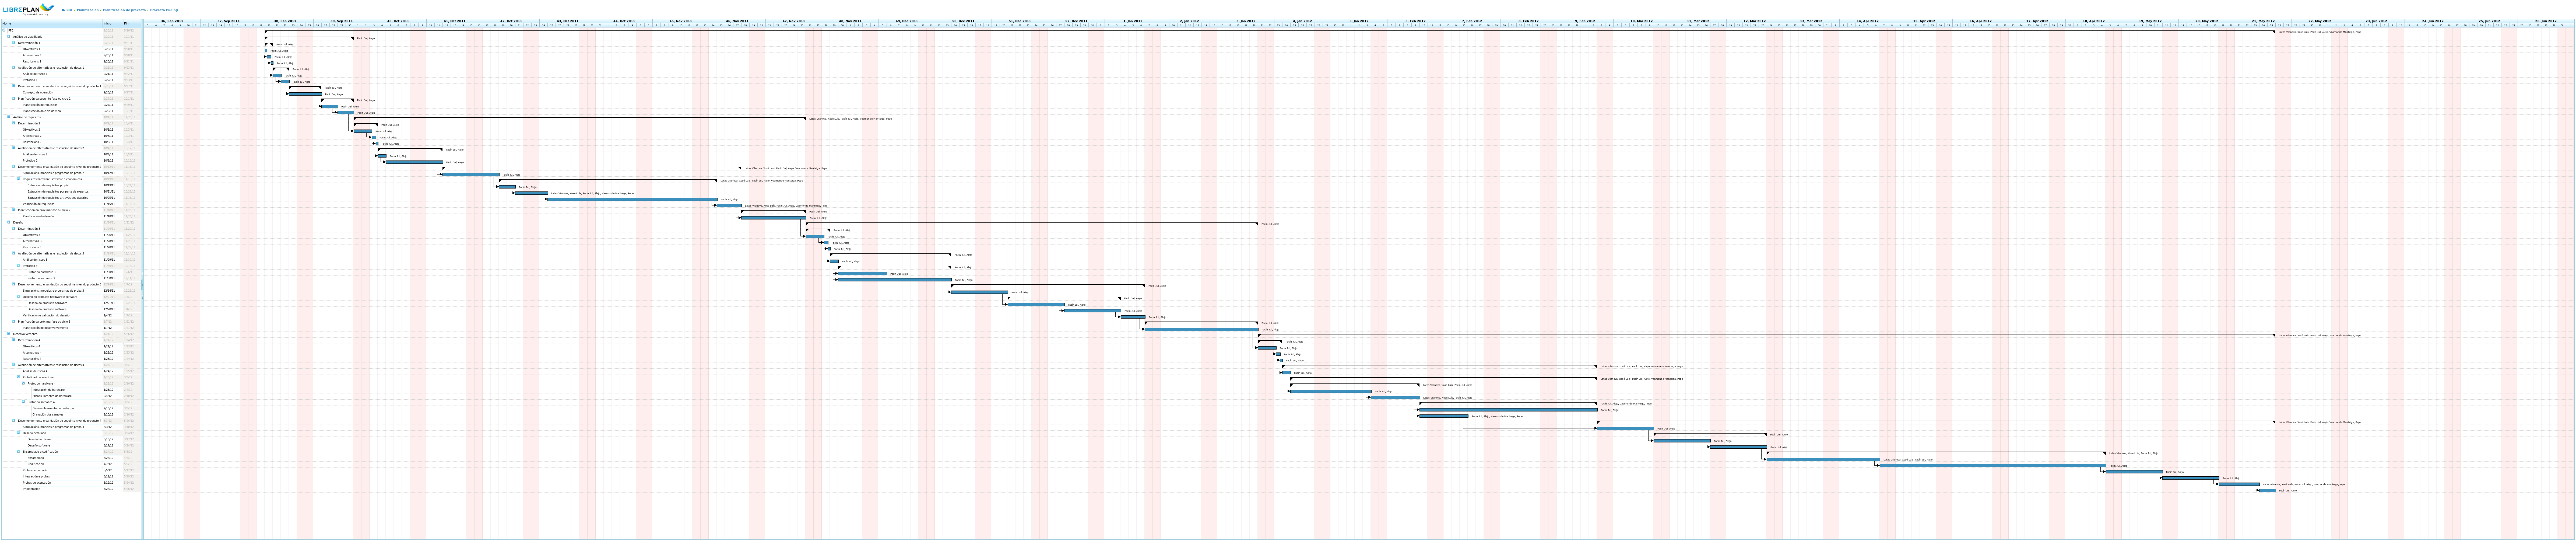
\includegraphics[trim=0 5cm 230cm 31cm,clip=true,scale=0.6,keepaspectratio=true]{./imagenes/planificacion-inicial.png}
 % planificacion-inicial.png: 9571x2035 pixel, 100dpi, 243.10x51.69 cm, bb=0 0 6891 1465
 \caption[Planificación inicial (2/2)]{Planificación inicial (2/2) \cite{LibrePlan}.}
 \label{figura:PlanificacionInicial2}
\end{figure}

A estimación da duración de cada tarefa contempla tanto o erro na propia
estimación coma os posibles desvíos derivados da análise de riscos e outros
imprevistos.\\

A modo de conclusión, comentar que ás veces merece a pena perder algo de tempo
probando unha ferramenta que se sabe que será de calidade, aínda que resulte
máis complexa, ca empregar outra máis sinxela pero con alta probabilidade de
fallo, como así aconteceu.